\documentclass{report}
\usepackage{graphicx}
\usepackage{xcolor}
\usepackage{natbib}

\begin{document}
\begin{titlepage}
	\begin{center}
	{\Huge\bfseries Rapport de Projet de Génie Logiciel\par}
	\vspace{1cm}
	{\huge\bfseries Tower Defense\par}
	\vspace{0.5cm}
	{\LARGE Anna Di Placido \par}
	\vspace{0.3cm}
	{\LARGE Markus Puura \par}
	
	\rule{12cm}{0.4pt} \newline
	\vspace{0.5cm}
	{\Large Master 1 Informatique\par}
	
	
	
	
	\vspace{2cm}
	
\includegraphics[width = 100mm]{logo-colonne-uca-couleur-master.png}
	\vfill
	{\large Novembre 2023 - Janvier 2024\par}
	\end{center}
\end{titlepage}


\newpage

\section*{1 Introduction}

Notre jeu de Tower Defense est codé avec Java sur Windows, en utilisant la librairie Swing. Pour coordonner notre travail nous avons utilisé GitHub et avant de commencer à coder nous avons réalisé un WBS pour déterminer les activités et sous-activités que nous aurons à réaliser pour avoir un jeu complet.

\section*{2 Fonctionnalités du jeu}
Pour jouer à notre jeu, il est nécessaire d'avoir Java 22 sur Windows. Pour lancer une partie, il suffit d'ouvrir le fichier execute.bat dans le dossier du jeu.\\
Le jeu est constitué de deux niveaux qui durent 5 minutes chacun, l'objectif est de défendre un château des monstres qui essayent de l'atteindre en plaçant des tours qui tuent ces derniers. Au début du niveau 1, le château possède 5 vies, à chaque monstre qui atteint le château, une vie est perdue, lorsque le niveau 1 se termine, le niveau 2 se lancera automatiquement, mais les vies perdues durant le niveau 1 ne sont pas régénérés.
\begin{figure}[!ht]
	\centering
	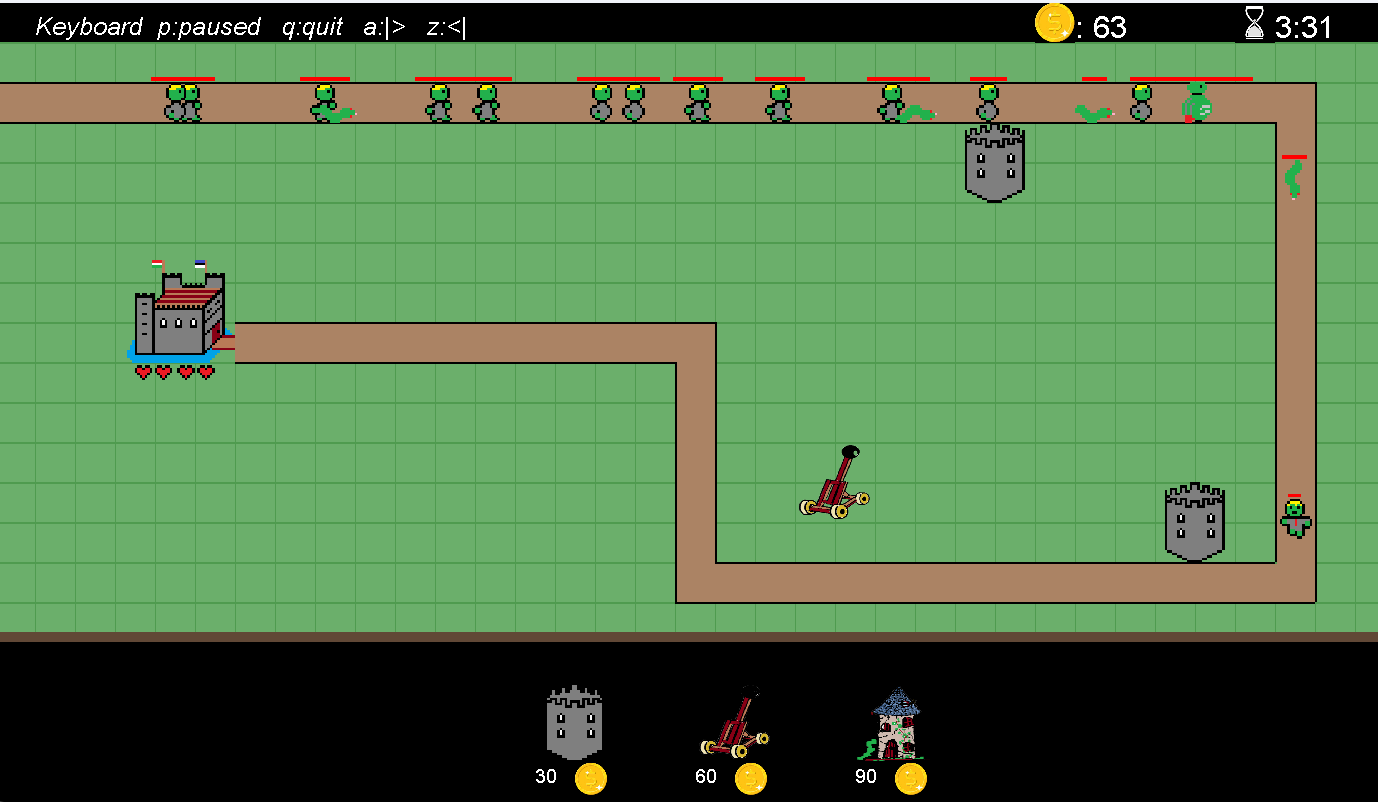
\includegraphics[scale=.5]{Jeu}
	\caption{Niveau 1 du jeu}
	\end{figure}
\\
Les fonctionnalités de notre jeu sont les suivantes:
\begin{itemize}
  \item Les monstres sont générés aléatoirement au début du chemin, mais à chaque minute qui passe, les chances d'apparition de monstres augmentent.
  \item Lorsqu'un monstre est tué, des pièces d'or sont récupérés par le joueur, dont la somme détenu est indiqué en haut à droite de l'écran, elles permettent de se procurer les tours de défense.
  \begin{figure}[!ht]
	\centering
	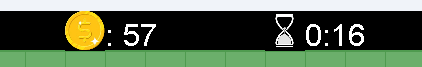
\includegraphics[scale=.8]{Pieces}
	\caption{Pièces récoltées + temps restant du niveau}
	\end{figure}
  \item Les tours disponibles à l'achat sont dans l'inventaire en bas de l'écran, accompagnés de leurs prix d'achat. Si le joueur possède assez de pièces pour acheter une tour, il peut cliquer sur cette tour, et la glisser au bord de la route dans une zone où il est autorisé à la placer, si le cercle autours de la tour est bleu, cela indique que le joueur a le droit de placer la tour à cette position, dans le cas contraire, le cercle est rouge. Le cercle indique aussi la portée des tirs de la tour. Lorsque le joueur relâche la clique, la tour est placée.
 \begin{figure}[!ht]
	\centering
	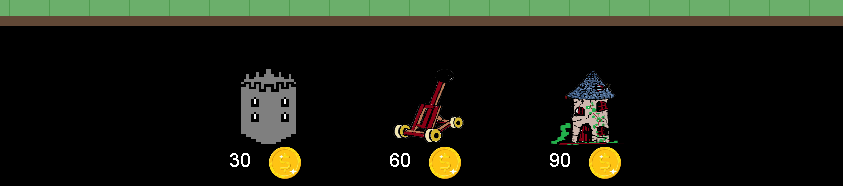
\includegraphics[scale=.7]{Inventaire}
	\caption{Inventaire des Tours à acheter}
	\end{figure}
	\begin{figure}[!ht]
	\centering
	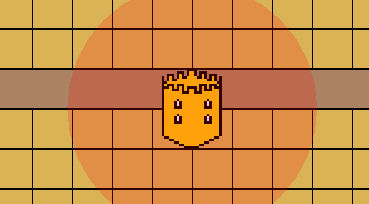
\includegraphics[scale=.7]{MalPlacé}
	\caption{Cercle rouge lorsque la tour ne peut pas être placée}
	\end{figure}
  \item Il est également possible d'augmenter le niveau d'une tour déjà placé, il suffit de cliquer dessus et de cliquer sur la flèche qui pointe vers le haut, le prix de cette augmentation est également indiqué, ces augmentations permettent d'augmenter la portée des tours et leurs vitesses de tir.
  
  \item Une tour peut également être vendu, en cliquant sur l'icône de pièce d'or après avoir sélectionné la tour, on récupère ensuite la somme de pièces indiqué sur ce bouton.
  \begin{figure}[!ht]
	\centering
	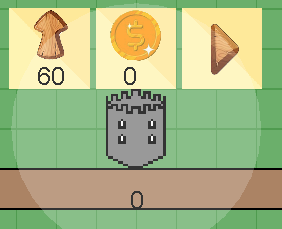
\includegraphics[scale=.5]{AmeliorationTour}
	\caption{Amélioration de la tour ou la vendre}
	\end{figure}
  \item Les différents tours ont des vitesses de tir, des portées et des dégâts infligés par tir différents. Le canon fait également des dégâts de zone, et la tour de sorcier permet de diviser par 2 la vitesse de tous les monstres qui s'en rapprochent.
  \item Les différents monstres ont également des caractéristiques qui différent, dont la vitesse, les points de vie, et les pièces récoltés en cas de mort. Le Golem fait apparaître 3 monstres plus petits et plus rapides lors de sa mort.
  \item Il est possible de mettre le jeu en pause en appuyant sur la touche p du clavier, de quitter la partie en appuyant sur q et de désactiver la musique de fond en cliquant sur m.
 
\end{itemize}
  
\section*{3 Model View Controller}

Le projet est organisé en MVC. Les modèles permettent de définir les attributs d’un objet ainsi que les fonctions qui seront appelés. La vue dessine le terrain de jeu ainsi que les images et les tire. Le controler permet d’interagir et d’envoyer les informations entre les modèles et la vue. Il sert d’intermédiaire entre la vue et le modèle.
Nos fichiers java sont séparés dans 3 répertoires différents: Modele, Vue et Controlleur, pour les séparer selon leur catégorie.


\section*{4 Design Patterns}

Nous avons employé cinq différents design patterns tout au long du projet:\\

\begin{itemize}
  \item \textbf{Iterator}: Nous avons une liste chaînée pour stocker et manipuler tous les monstres qui sont vivants tout au long de la partie. Lorsqu'un monstre est généré, il est ajouté dans la liste, et lorsqu'il meurt, il est retiré. Et après chaque mise à jour de la partie, pour tous les tours qui ont été placés, cette liste est parcouru pour enlever les dégâts infligés par les tours au/aux monstre(s) concernés. Pour faire avancer tous les monstres, la liste est également parcourue après chaque mise à jour.
  \item \textbf{Factory}: pour avoir une modularité et une flexibilité dans la conception des tours du jeu, nous avons utilisé la Factory qui a permit de regrouper tous les types de projectiles.
L’énumération ProjectileType.java regroupe les types: TOUR, CANON et TOUR\textunderscore SORCIER.
La Factory ProjectileFactory crée une instance de projectile selon le type énuméré en paramètre d’une fonction.
Cela est utilisé dans le controller MouseController lorsque l’utilisateur interagit avec la souris pour sélectionner un des projectiles à créer. Par exemple avec le choix de la tour dans la barre d’inventaire, la Factory utilise le type TOUR pour créer une instance de Tour1.java avec ses paramètres lorsqu’elle est déposée sur le plateau de jeu.
	\item \textbf{Strategy}: L’interface Strategy est commune à toutes les stratégies de tire pour chaque projectile, elle déclare une méthode que les projectiles utilisent pour leur tire.
DirectShoot, RallentirShoot et ZonedShoot implémentent la fonction de l’interface de différentes manières.
Chaque projectile crée un objet de ShootStrategy et applique le type de tire sur les monstres. Cela permet de regrouper toutes les tires possibles en les mettant dans des classes séparées et de rendre leurs objets interchangeables: la tour effectue des dégâts seulement sur un personnage a la fois. Le Canon fait des dégâts de zone. La Tour sorcier ralentis les personnages dans un certain rayon.\\
\begin{figure}[!ht]
	\centering
	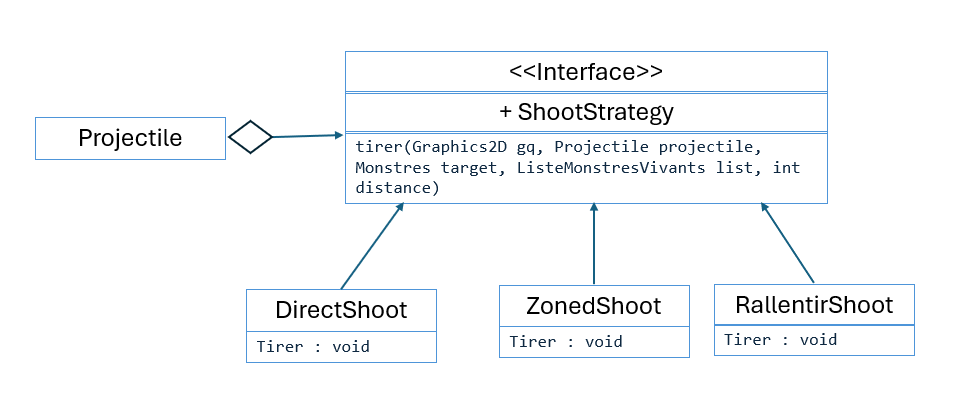
\includegraphics[scale=.5]{Strategy}
	\caption{Design Pattern Strategy}
	\end{figure}
	
	\item \textbf{Singleton}: Le château à la fin du chemin est représenté comme singleton, car il est unique dans le jeu.
Tunel.java dans notre jeu crée une instance unique pour la tour avec ses vies qui diminuent lorsqu’un monstre entre dans sa zone.
Cela permet de garder le même nombre de vies restantes lorsque le jeu passe du niveau 1 au niveau 2.
	\item \textbf{Abstract Factory}: Nous avons des classes abstraites pour avoir des interfaces pour créer des familles d'objets liés ou dépendants sans spécifier leurs classes concrètes. Nous les utilisons pour créer les différents monstres (Monstres.java) et les différentes tours (Projectile.java).
	
\section*{5 Conclusion}

Notre jeu était assez fournis pour avoir du travail tout au long du temps imparti. Le travail était bien réparti dans notre équipe.\\
Si nous devions continuer ce jeu, il serait intéressant d'ajouter encore des niveaux supplémentaires avec de nouveaux mondes et de nouveaux monstres. Et peut être ajouté de nouvelles tours avec de nouvelles capacités.

\end{itemize}


\end{document}